    \item Four points $\vec{P}\brak{0, 1}$, $\vec{Q}\brak{0, -3}$, $\vec{R}\brak{-2, -1}$, and $\vec{S}\brak{2, -1}$ represent the vertices of a quadrilateral.
    What is the area enclosed by the quadrilateral?
    \hfill{(EC 2022)}
    \begin{enumerate}
        \begin{multicols}{4}
        \item 4
        \item $4\sqrt{2}$
        \item 8
        \item $8\sqrt{2}$
        \end{multicols}
    \end{enumerate}
    \item Consider the following square in \figref{fig:m3} with the four corners and the center marked as P, Q, R, S and T respectively.
    \begin{figure}[H]
        \centering
        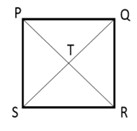
\includegraphics[width=0.25\columnwidth]{GATE/2022/EC/figs/m3.jpg}
        \caption{}
        \label{fig:m3}
    \end{figure}
    Let X, Y and Z represent the following operations:
	    \begin{enumerate}[label=\Alph*:, start=24]
    
\item rotation of the square by 180 degree with respect to the S-Q axis.
\item rotation of the square by 180 degree with respect to the P-R axis.
\item rotation of the square by 90 degree clockwise with respect to the axis perpendicular, going into the screen and passing through the point T.
\end{enumerate}
    Consider the following three distinct sequences of operation \brak{\text{which are applied in the left to right order}}.
    \begin{enumerate}[label=(\arabic*)]
        \item XYZZ
        \item XY
        \item ZZZZ
    \end{enumerate}
    Which one of the following statements is correct as per the information provided above?
    \hfill{(EC 2022)}
    \begin{enumerate}
        \item The sequence of operations \brak{1} and \brak{2} are equivalent
        \item The sequence of operations \brak{1} and \brak{3} are equivalent
        \item The sequence of operations \brak{2} and \brak{3} are equivalent
        \item The sequence of operations \brak{1}, \brak{2} and \brak{3} are equivalent
    \end{enumerate}
    \item Consider a system of linear equations $\vec{A}\vec{x} = \vec{b}$, where
    \begin{align*}
	    \vec{A} = \myvec{1 & -\sqrt{2} \\ -1 & \sqrt{2}},  \vec{b} = \myvec{1 \\ 3}
    \end{align*}
    This system of equations admits \rule{2cm}{0.4pt}.
    \hfill{(EC 2022)}
    \begin{enumerate}
    \begin{multicols}{2}
        \item a unique solution for $\vec{x}$
        \item infinitely many solutions for $\vec{x}$
        \item no solutions for $\vec{x}$
        \item exactly two solutions for $\vec{x}$
        \end{multicols}
    \end{enumerate}
    \item Let $\alpha, \beta$ be two non-zero real numbers and $\vec{v}_1, \vec{v}_2$ be two non-zero real vectors of size $3 \times 1$. Suppose that $\vec{v}_1$ and $\vec{v}_2$ satisfy $\vec{v}_1^{\top} \vec{v}_2 = 0$, $\vec{v}_1^{\top} \vec{v}_1 = 1$, and $\vec{v}_2^{\top} \vec{v}_2 = 1$. Let $\vec{A}$ be the $3 \times 3$ matrix given by:
    \begin{align*}
     \vec{A} = \alpha \vec{v}_1 \vec{v}_1^{\top} + \beta \vec{v}_2 \vec{v}_2^{\top} 
     \end{align*}
    The eigenvalues of $\vec{A}$ are \rule{2cm}{0.4pt}.
    \hfill{(EC 2022)}
    \begin{enumerate}
    \begin{multicols}{4}
        \item $0, \alpha, \beta$
        \item $0, \alpha+\beta, \alpha-\beta$
        \item $0, \frac{\alpha+\beta}{2}, \sqrt{\alpha\beta}$
        \item $0, 0, \sqrt{\alpha^2+\beta^2}$
        \end{multicols}
    \end{enumerate}
